\documentclass[12pt,addpoints]{repaso}
\grado{3}
\nivel{Secundaria}
\cicloescolar{2024-2025}
\materia{Ciencias y Tecnología: Química \normalfont \color{darkgray}\small con adecuación curricular}
\unidad{3}
\title{Practica la Unidad}
\aprendizajes{\footnotesize%
        \item Analiza el aporte energético de los alimentos y lo relaciona con las actividades físicas personales, a fin de tomar decisiones vinculadas a una dieta saludable. 
        \item Distingue las propiedades de ácidos y bases en su entorno, a partir de indicadores e interpreta la escala de acidez y basicidad. 
        \item Explica los factores que influyen en la rapidez de las reacciones químicas, con base en la identificación y control de variables mediante actividades experimentales y modelos corpusculares.
        \item Identifica reacciones de óxido-reducción en su entorno y comprende su importancia en diferentes ámbitos.  
}
\author{Melchor Pinto, J.C.}
\begin{document}
\INFO%
\begin{questions}
    \questionboxed[12]{ Relaciona las representaciones del modelo cin\'etico de part\'iculas con el tipo de materia que le corresponda:\\

        \begin{center}\Large
            \wordpill{Compuesto} \wordpill{Elemento} \wordpill{Mezcla}
        \end{center}

        \begin{multicols}{3}
            \begin{parts}
                \part \begin{minipage}[t]{\linewidth}
                    \raggedright
                    \adjustbox{valign=b}{%
                        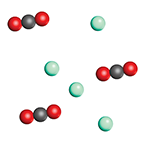
\includegraphics[width =0.5\textwidth ]{mezcla1.png}
                    }
                    \rule{2cm}{0.2mm}
                \end{minipage}
                \part \begin{minipage}[t]{\linewidth}
                    \raggedright
                    \adjustbox{valign=b}{%
                        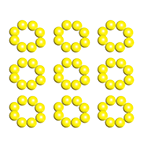
\includegraphics[width =0.5\textwidth ]{elemento1.png}
                    }
                    \rule{2cm}{0.2mm}
                \end{minipage}
                \part \begin{minipage}[t]{\linewidth}
                    \raggedright
                    \adjustbox{valign=b}{%
                        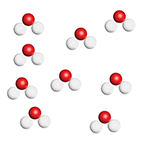
\includegraphics[width =0.5\textwidth ]{compuesto2.png}
                    }
                    \rule{2cm}{0.2mm}
                \end{minipage}
                \part \begin{minipage}[t]{\linewidth}
                    \raggedright
                    \adjustbox{valign=b}{%
                        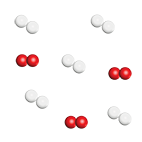
\includegraphics[width =0.5\textwidth ]{mezcla2.png}
                    }
                    \rule{2cm}{0.2mm}
                \end{minipage}
                \part \begin{minipage}[t]{\linewidth}
                    \raggedright
                    \adjustbox{valign=b}{%
                        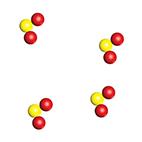
\includegraphics[width =0.5\textwidth ]{compuesto1.png}
                    }
                    \rule{2cm}{0.2mm}
                \end{minipage}
                \part \begin{minipage}[t]{\linewidth}
                    \raggedright
                    \adjustbox{valign=b}{%
                        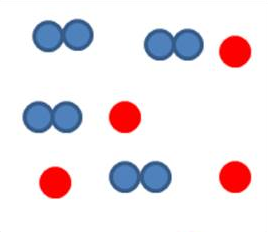
\includegraphics[width =0.5\textwidth ]{mezcla3.png}
                    }
                    \rule{2cm}{0.2mm}
                \end{minipage}
                \part \begin{minipage}[t]{\linewidth}
                    \raggedright
                    \adjustbox{valign=b}{%
                        
\includegraphics[width =0.5\textwidth ]{elemento3.png}
                    }
                    \rule{2cm}{0.2mm}
                \end{minipage}
                \part \begin{minipage}[t]{\linewidth}
                    \raggedright
                    \adjustbox{valign=b}{%
                        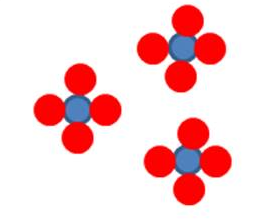
\includegraphics[width =0.5\textwidth ]{compuesto3.png}
                    }
                    \rule{2cm}{0.2mm}
                \end{minipage}
                \part \begin{minipage}[t]{\linewidth}
                    \raggedright
                    \adjustbox{valign=b}{%
                        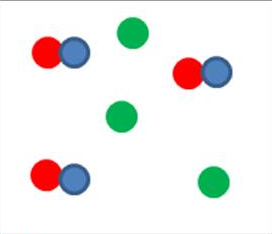
\includegraphics[width =0.5\textwidth ]{mezcla4.png}
                    }
                    \rule{2cm}{0.2mm}
                \end{minipage}
                % \part \begin{minipage}[t]{\linewidth}
                %     \raggedright
                %     \adjustbox{valign=b}{%
                %         
\includegraphics[width =0.5\textwidth ]{elemento2.png}
                %     }
                %     \rule{2cm}{0.2mm}
                % \end{minipage}
                \part \begin{minipage}[t]{\linewidth}
                    \raggedright
                    \adjustbox{valign=b}{%
                        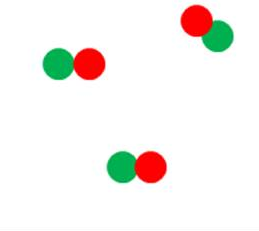
\includegraphics[width =0.5\textwidth ]{compuesto4.png}
                    }
                    \rule{2cm}{0.2mm}
                \end{minipage}
                \part \begin{minipage}[t]{\linewidth}
                    \raggedright
                    \adjustbox{valign=b}{%
                        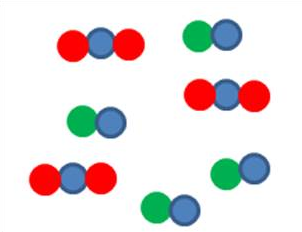
\includegraphics[width =0.5\textwidth ]{mezcla5.png}
                    }
                    \rule{2cm}{0.2mm}
                \end{minipage}
                \part \begin{minipage}[t]{\linewidth}
                    \raggedright
                    \adjustbox{valign=b}{%
                        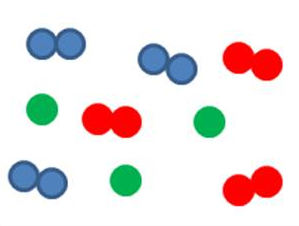
\includegraphics[width =0.5\textwidth ]{mezcla6.png}
                    }
                    \rule{2cm}{0.2mm}
                \end{minipage}

            \end{parts}
        \end{multicols}
    }

    \questionboxed[10]{Anota una \checkmark \ en el recuadro correspondiente en cada afirmación.

        \begin{table}[H]
            \centering
            \resizebox{0.8\textwidth}{!}{%
                \begin{tabular}{|l|c|c|}
                    \hline
                    \textbf{Las vacunas pueden ocasionar \dots}                          & \textbf{Mito}                             & \textbf{Efecto secundario}                \\ \hline
                    malestar general y dolor de cabeza.                                  &                                           & \ifprintanswers{\color{red}\checkmark}\fi \\ \hline
                    cambios menstruales y sangrado vaginal inesperado.                   &                                           & \ifprintanswers{\color{red}\checkmark}\fi \\ \hline
                    alteraciones en la estructura del adn de las personas.               & \ifprintanswers{\color{red}\checkmark}\fi &                                           \\ \hline
                    un incremento en la tasa de morbilidad y mortalidad.                 & \ifprintanswers{\color{red}\checkmark}\fi &                                           \\ \hline
                    una viremia leve, que puede provocar erupción cutánea.               &                                           & \ifprintanswers{\color{red}\checkmark}\fi \\ \hline
                    afecciones neurológicas, como los trastornos del espectro autista.   & \ifprintanswers{\color{red}\checkmark}\fi &                                           \\ \hline
                    el desarrollo de nuevas variantes del virus que causa la enfermedad. & \ifprintanswers{\color{red}\checkmark}\fi &                                           \\ \hline
                    enrojecimiento, hinchazón y algunos síntomas sistémicos como fiebre. &                                           & \ifprintanswers{\color{red}\checkmark}\fi \\ \hline
                \end{tabular}
            }
        \end{table}
    }

    \questionboxed[12]{Marca las alternativas que consideres necesarias para reducir las muertes por la contaminación del aire.

        % \begin{multicols}{2}
        \begin{checkboxes}
            \CorrectChoice Favorecer el uso de fuentes de energía menos contaminantes, como el gas natural.
            \choice Promover el uso de combustibles sólidos como fuente de energía doméstica.
            \CorrectChoice Incentivar el uso de la bicicleta y el desarrollo de un transporte público sostenible
            \choice Impulsar leyes y políticas que favorezcan el uso de precursores de ozono.
            \CorrectChoice Fomentar una ventilación adecuada entre los hogares de ingresos más bajos.
        \end{checkboxes}
        % \end{multicols}
    }

    \questionboxed[10]{Anota una \checkmark \ en las acciones que crees que pueden mejorar la gestión de los desechos.

        \begin{table}[H]
            \centering
            \resizebox{0.8\textwidth}{!}{%
                \begin{tabular}{|l|c|}
                    \hline
                    Evitar al mínimo utilizar plásticos de un solo uso.            & \hspace{2cm} \\ \hline
                    No quemar la basura.                                           & \hspace{2cm} \\ \hline
                    No tirar la basura en el drenaje, cuerpos de agua o barrancas. & \hspace{2cm} \\ \hline
                    Separar de forma adecuada la basura.                           & \hspace{2cm} \\ \hline
                    Reducir, reutilizar y reciclar.                                & \hspace{2cm} \\ \hline
                    Donar los objetos o ropa que no utilices.                      & \hspace{2cm} \\ \hline
                    Desechar en contenedores especiales las pilas y las baterías.  & \hspace{2cm} \\ \hline
                    Desecho responsable de equipos electrónicos.                   & \hspace{2cm} \\ \hline
                    Reflexionar acerca de lo que compro: ¿realmente lo necesito?   & \hspace{2cm} \\ \hline
                \end{tabular}
            }
        \end{table}
    }

    \questionboxed[8]{Relaciona cada elemento con su función en el cuerpo humano.\\

        % \begin{multicols}{2}
        \begin{minipage}{0.2\textwidth}
            \begin{choices}\large
                \choice Hierro
                \choice Calcio
                \choice Nitrógeno
                \choice Potasio
            \end{choices}
        \end{minipage} % \columnbreak%
        \begin{minipage}{0.8\textwidth}
            \begin{parts}\normalsize
                \part \fillin[B][1cm] Mantiene los huesos y dientes sanos y fuertes.
                \part \fillin[C][1cm] Forma parte de los aminoácidos (que componen las proteínas) y de los ácidos nucleicos (ADN y ARN).
                \part \fillin[A][1cm] Produce hemoglobina, una proteína que transporta el oxígeno de los pulmones a distintas partes del cuerpo humano.
                \part \fillin[D][1cm] Relaja el músculo tras una contracción.
            \end{parts}
        \end{minipage}
        % \end{multicols}

    }

    \questionboxed[10]{Selecciona las respuestas correctas con base en tus conocimientos.

        \begin{multicols}{2}
            \begin{parts}
                \part ¿Qué es la seguridad alimentaria?

                \begin{choices}
                    \choice La disponibilidad de alimentos en un determinado país.
                    \choice La calidad y la sostenibilidad de los alimentos disponibles.
                    \choice El acceso económico a los alimentos por parte de la población.
                    \choice El acceso físico, social y económico a alimentos suficientes, seguros y nutritivos.
                \end{choices}

                \part ¿Por qué es esencial para nuestro organismo beber agua potable todos los días?

                \begin{choices}
                    \choice Humecta las mucosas.
                    \choice Mantiene una buena salud digestiva.
                    \choice Mantiene el flujo sanguíneo.
                    \choice Todas las anteriores.
                \end{choices}

                \part ¿Qué nutrimentos aportan los cereales integrales?

                \begin{oneparchoices}
                    \choice Agua
                    \choice Minerales \\
                    \choice Vitaminas
                    \choice Todos los anteriores
                \end{oneparchoices}

                \part ¿Cuánto tiempo puede vivir una persona sin beber agua?

                \begin{oneparchoices}
                    \choice 2 meses
                    \choice Tres semanas \\
                    \choice 1.5 años
                    \choice Unos cuantos días
                \end{oneparchoices}

                \part¿En qué grupos la desigualdad alimentaria y los problemas de salud son más pronunciados?

                \begin{choices}
                    \choice Zonas rurales
                    \choice Pueblos indígenas
                    \choice Áreas campesinas
                    \choice Todos las anteriores
                \end{choices}
            \end{parts}
        \end{multicols}
    }

    \questionboxed[10]{Marca los recuadros correspondientes a los riesgos y las enfermedades asociadas al consumo de alimentos procesados cuyos empaques incluyen estos sellos.

        \begin{minipage}{0.4\textwidth}
            \begin{center}
                
\includegraphics[width=0.8\linewidth]{img0001.png}
            \end{center}
        \end{minipage}%
        \begin{minipage}{0.6\textwidth}
            \begin{multicols}{2}
                \begin{checkboxes}\large
                    \choice Salmonela
                    \choice Obesidad
                    \CorrectChoice Caries

                    \columnbreak%

                    \choice Enfisema
                    \CorrectChoice Sobrepeso
                    \CorrectChoice Diabetes
                \end{checkboxes}
            \end{multicols}
        \end{minipage}
    }



    \questionboxed[6]{Contesta, con base en la información anterior y tus conocimientos.

        \begin{center}
            \resizebox{0.8\textwidth}{!}{%
                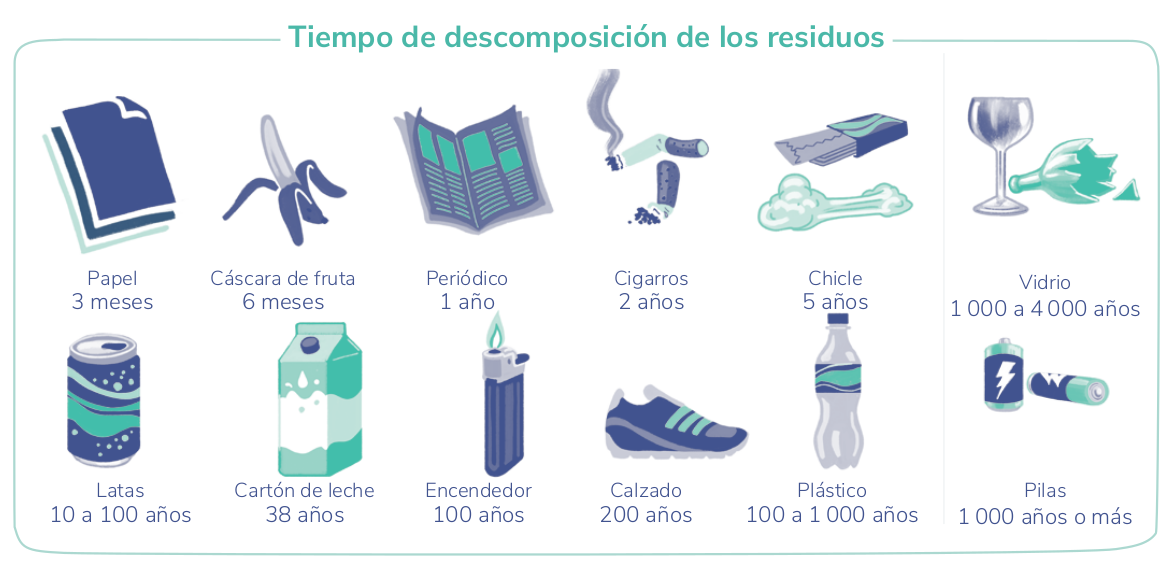
\includegraphics{img0002.png}
            }
        \end{center}

        \begin{parts}
            \part ¿Cuánto tiempo tardan en descomponerse los residuos relacionados con los alimentos?

            \begin{solutionbox}{3cm}
                Cáscara de frutas, 6 meses; latas, 10 a 100 años; cartón de leche, 38 años; plástico, 100 a 1 000
                años; vidrio, 1 000 a 4 000 años.
            \end{solutionbox}
            \part ¿Cómo se aprovechan en la actualidad los residuos que pueden tardar 1 000 años o más en
            descomponerse?
            \begin{solutionbox}{3cm}
                El plástico se descompone térmicamente en ausencia de oxígeno para obtener sustancias
                que se usan como combustibles. El vidrio se tritura y se funde para fabricar nuevos materiales de
                vidrio. Los componentes metálicos de las baterías, como el litio, el cobalto o el níquel, se extraen
                y se reciclan para su reutilización en nuevas baterías o en otros productos.
            \end{solutionbox}
            \part ¿Cuáles son las razones por las que algunos materiales se degradan más rápido que otros?
            \begin{solutionbox}{3cm}
                Tienen diferente tiempo de degradación, porque están constituidos por diversos materiales,
                los cuales tienen distintas características y propiedades físicas y químicas. Por otra parte, también
                influye el entorno en el que se encuentre, es decir, si está al aire libre o se encuentra en un relleno
                sanitario.
            \end{solutionbox}

        \end{parts}
    }

    \begin{multicols}{2}
        \ejemplosboxed[\include*{../questions/question026e}]

        \questionboxed[10]{\include*{../questions/question026l}}
    \end{multicols}

    \questionboxed[12]{Anota una \checkmark \ en las actividades físicas en las que el gasto de energía por hora es mayor a 300 Cal.\\

        \begin{multicols}{3}
            \begin{checkboxes}\large
                \choice Ver televisión
                \CorrectChoice Nadar
                \choice Leer
                \CorrectChoice Bailar
                \choice Andar en bicicleta
                \CorrectChoice Subir escaleras
                \CorrectChoice Correr
                \choice Caminar
                \CorrectChoice Jugar basquetbol
                \choice Tender la cama
                \choice Jugar voliebol
                \CorrectChoice Jugar futbol
            \end{checkboxes}
        \end{multicols}
    }
\end{questions}
\end{document}

